\section{Quantities and Units}
\label{sec:Quantities}
%%%%%%%%%%%%%%%%%%%%%%%%%%%%%%%%%%%%%%%%%%%%%%%%%%%%%%%%
\begin{figure}[h!]
\begin{center}
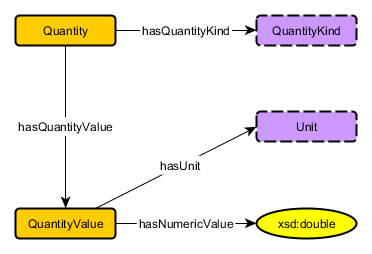
\includegraphics[width=.7\textwidth]{figures/quantities}
\end{center}
\caption{Schema Diagram for Quantities and Units.}
\label{fig:Quantities}
\end{figure}
\subsection{Summary}
\label{sum:Quantities}
%%%%%%%%%%%%%%%%%%%%%%%%%%%%
This pattern is heavily adapted from QUDT\footnote{\url{http://www.qudt.org/release2/qudt-catalog.html}}. A \textsf{Quantity} 

Reification?

\textsf{QuantityKind} and \textsf{Unit} are controlled vocabularies, as recommended by QUDT \cite{qudt}.

%%%%%%%%%%%%%%%%%%%%%%%%%%%%%%%%%%%%%%%%%%%%%%%%%%%%%%%%
\subsection{Axiomatization}
\label{axs:Quantities}
%%%%%%%%%%%%%%%%%%%%%%%%%%%%
\begin{align}
\top &\sqsubseteq \forall \textsf{hasQuantityKind.QuantityKind} \\
\top &\sqsubseteq \forall \textsf{hasQuantityValue.QuantityValue} \\
\top &\sqsubseteq \forall \textsf{hasUnit.Unit} \\
\top &\sqsubseteq \forall \textsf{hasNumericaValue.xsd:double}
\end{align}

%%%%%%%%%%%%%%%%%%%%%%%%%%%%%%%%%%%%%%%%%%%%%%%%%%%%%%%%
\subsection{Explanations}
\label{exp:Quantities}
%%%%%%%%%%%%%%%%%%%%%%%%%%%%
\begin{enumerate}
\item Range: the range of \textsf{hasQuantityKind} is \textsf{QuantityKind}.
\item Range: the range of \textsf{hasQuantityValue} is \textsf{QuantityValue}.
\item Range: the range of \textsf{hasUnit} is \textsf{Unit}.
\item Range: the range of \textsf{hasNumericValue} is \textsf{xsd:double}.
\end{enumerate}

%%%%%%%%%%%%%%%%%%%%%%%%%%%%%%%%%%%%%%%%%%%%%%%%%%%%%%%%
\subsection{Competency Question}
\label{cqs:Quantities}
%%%%%%%%%%%%%%%%%%%%%%%%%%%%
\begin{enumerate}[CQ1.]
\item How much does an elephant weigh in kilograms?
\item How long is Jupiter from the Sun, at its farthest, in furlongs?
\end{enumerate}

\newpage
%%%%%%%%%%%%%%%%%%%%%%%%%%%%%%%%%%%%%%%%%%%%%%%%%%%%%%%%
% End Section
%%%%%%%%%%%%%%%%%%%%%%%%%%%%%%%%%%%%%%%%%%%%%%%%%%%%%%%%
%%%%%%%%%%%%%%%%%%%%%%%%%%%%%%%%%%%%%%%%%%%%%%%%%%%%%%%%